%%%%%%%%%%%%%%%%%%%%%%%%%%%%%%%%%%%%%%%%%%%%%%%%%%%%%%%%%%%%%%%%%%%%%%%%%%%%%%%%
%2345678901234567890123456789012345678901234567890123456789012345678901234567890
%        1         2         3         4         5         6         7         8

%\documentclass[journal,transmag]{IEEEtran}% Comment this line out if you need a4paper

\documentclass[10pt, conference]{ieeeconf}      % Use this line for a4 paper


\IEEEoverridecommandlockouts                              % This command is only needed if 
                                                          % you want to use the \thanks command

%\overrideIEEEmargins                                      % Needed to meet printer requirements.

% See the \addtolength command later in the file to balance the column lengths
% on the last page of the document

% The following packages can be found on http:\\www.ctan.org
%\usepackage{graphics} % for pdf, bitmapped graphics files
%\usepackage{epsfig} % for postscript graphics files
%\usepackage{mathptmx} % assumes new font selection scheme installed
%\usepackage{times} % assumes new font selection scheme installed
%\usepackage{amsmath} % assumes amsmath package installed
%\usepackage{amssymb}  % assumes amsmath package installed

\newtheorem{theorem}{Theorem}[section]
\newtheorem{lemma}[theorem]{Lemma}
\newtheorem{proposition}[theorem]{Proposition}
\newtheorem{corollary}[theorem]{Corollary}
\usepackage[ruled,vlined]{algorithm2e}
\usepackage{url}
\newenvironment{definition}[1][Definition]{\begin{trivlist}
\item[\hskip \labelsep {\bfseries #1}]}{\end{trivlist}}

\newcommand{\qed}{\nobreak \ifvmode \relax \else
      \ifdim\lastskip<1.5em \hskip-\lastskip
      \hskip1.5em plus0em minus0.5em \fi \nobreak
      \vrule height0.75em width0.5em depth0.25em\fi}

\def\lc{\left\lfloor}   
\def\rc{\right\rfloor}

\usepackage{amsmath,amssymb}

\usepackage{tabularx}
\usepackage{tikz,hyperref,graphicx,units}
\usepackage{subfigure}
\usepackage{benktools}
\usepackage{bbm}
\renewcommand{\baselinestretch}{.5}

\usepackage{caption}
\usepackage{epstopdf}
\renewcommand{\captionfont}{\footnotesize}
\usepackage{sidecap,wrapfig}
\usepackage[ruled,vlined]{algorithm2e}
\DeclareMathOperator*{\argmin}{arg\,min}
\DeclareMathOperator*{\argmax}{arg\,max}
\newcommand{\abs}[1]{\lvert#1\rvert} 
\newcommand{\norm}[1]{\lVert#1\rVert}
%\newcommand{\suchthat}{\mid}
\newcommand{\suchthat}{\ \big|\ }
\newcommand{\ba}{\mathbf{a}}
\newcommand{\bb}{\mathbf{b}}
\newcommand{\bc}{\mathbf{c}}
\newcommand{\bd}{\mathbf{d}}
\newcommand{\bg}{\mathbf{g}}
\newcommand{\bj}{\mathbf{j}}
\newcommand{\bn}{\mathbf{n}}
\newcommand{\bp}{\mathbf{p}}
\newcommand{\bw}{\mathbf{w}}
\newcommand{\bt}{\mathbf{t}}
\newcommand{\bu}{\mathbf{u}}
\newcommand{\by}{\mathbf{y}}
\newcommand{\bx}{\mathbf{x}}
\newcommand{\bz}{\mathbf{z}}
\newcommand{\bbf}{\mathbf{f}}
\newcommand{\bzero}{\mathbf{0}}
\newcommand{\bG}{\mathbf{G}}
\newcommand{\bA}{\mathbf{A}}
\newcommand{\bW}{\mathbf{W}}
\newcommand{\bX}{\mathbf{X}}
\newcommand{\mX}{\mathcal{X}}
\newcommand{\mD}{\mathcal{D}}
\newcommand{\mG}{\mathcal{G}}
\newcommand{\mN}{\mathcal{N}}
\newcommand{\mW}{\mathcal{W}}
\newcommand{\mF}{\mathcal{F}}
\newcommand{\bZ}{\mathbf{Z}}
\newcommand{\mR}{\mathcal{R}}

\newcommand{\bfc}{W}
\newcommand{\Qinf}{Q_{\infty}}
\newcommand{\st}[1]{_\text{#1}}
\newcommand{\rres}{r\st{res}}
\newcommand{\pos}[1]{(#1)^+}
\newcommand{\depth}{\operatorname{depth}}
\newcommand{\dist}{\operatorname{dist}}
\newcommand{\convhull}{\operatorname{ConvexHull}}
\newcommand{\minksum}{\operatorname{MinkowskiSum}}

\newcommand{\specialcell}[2][c]{ \begin{tabular}[#1]{@{}c@{}}#2\end{tabular}}
\newcommand{\acro}{SHIV}
\newcommand\independent{\protect\mathpalette{\protect\independenT}{\perp}}
\def\independenT#1#2{\mathrel{\rlap{$#1#2$}\mkern2mu{#1#2}}}

\newcolumntype{L}[1]{>{\RaggedRight\hspace{0pt}}p{#1}}
\newcolumntype{R}[1]{>{\RaggedLeft\hspace{0pt}}p{#1}}


\newboolean{include-notes}
\setboolean{include-notes}{true}
\newcommand{\adnote}[1]{\ifthenelse{ \boolean{include-notes}}%
 {\textcolor{blue}{\textbf{AD: #1}}}{}}
 
 \newcommand{\fpnote}[1]{\ifthenelse{ \boolean{include-notes}}%
 {\textcolor{blue}{\textbf{FP: #1}}}{}}
 
  \newcommand{\mlnote}[1]{\ifthenelse{ \boolean{include-notes}}%
 {\textcolor{purple}{\textbf{ML: #1}}}{}}

\renewcommand{\baselinestretch}{.95}
\usepackage{times}
\usepackage{microtype}
%\title{Iterative Imitation Learning with Reduced Human Supervision [v11]}
%\title{SHIV:  Reducing Human Supervision for Robot Active Learning [v11]}

\title{Robotic Grasping in Clutter: Using a Hierarchy of Supervisors with Learning from Demonstrations}



\author{Michael Laskey$^1$, Jonathan Lee$^1$, Caleb Chuck$^1$, David Gealy$^1$, Wesley Hsieh$^1$, Florian T. Pokorny,\\
 Anca D. Dragan$^1$, and Ken Goldberg$^{1,2}$% <-this % stops a space
\thanks{$^1$ Department of Electrical Engineering and Computer Sciences; {\small \{mdlaskey,iamwesleyhsieh,ftpokorny,anca\}@berkeley.edu} }%
\thanks{$^2$ Department of Industrial Engineering and Operations Research; {\small goldberg@berkeley.edu}}%
\thanks{$^{1-2}$ University of California, Berkeley;  Berkeley, CA 94720, USA}%
}
\begin{document}



\maketitle
\thispagestyle{empty}
\pagestyle{empty}


%%%%%%%%%%%%%%%%%%%%%%%%%%%%%%%%%%%%%%%%%%%%%%%%%%%%%%%%%%%%%%%%%%%%%%%%%%%%%%%%

\begin{abstract}
For applications such as Amazon warehouse order fulfillment, robots must grasp a desired object amid clutter: other
objects that block direct access.  This can be difficult to program explicitly due to uncertainty in friction and push
mechanics and the large number of objects that can be encountered. Online Learning from Demonstration (LfD) algorithms
such as DAgger and SHIV have potential to learn robot control policies for tasks where the system dynamics and the cost
function are unknown. To reduce the burden on human experts to provide control demonstrations, we propose using a
hierarchy of supervisors and a Deep Learning network to learn a grasping in clutter task.  We consider 3 levels of
supervisors, a fast motion planner that ignores obstacles, crowdsourced human workers who
provide appropriate robot control values via online videos, and local human experts.  Experiments suggest that we can
leverage a hiearchy of supervisors to obtain 22,000 labelled training data examples and achieve 80\% success on a held out test set of unknown objects.

 \end{abstract}


%%%%%%%%%%%%%%%%%%%%%%%%%%%%%%%%%%%%%%%%%%%%%%%%%%%%%%%%%%%%%%%%%%%%%%%%%%%%%%%%

\section{Introduction} 
As illustrated by the recent Amazon Picking Challenge at ICRA 2015, the grasping in clutter problem, where a robot needs
to grasp an object that might be occluded by other objects in the environment poses an interesting challenge to robotic
systems. This problem is relevant to industrial applications such as warehouse shipping operations and flexible manufacturing in a semi-structured environments. One fundamental approach to grasping in clutter is the analytic model driven approach~\cite{bicchi2000robotic},
where the interaction dynamics between the robot and obstacles are formulated analytically. However, modeling all the 
physical properties of interaction poses a highly challenging problem due to uncertainty in modeling parameters such as
inertial properties and friction. 

Another approach to the grasping in
clutter problem is a data-driven manner, where the interaction behavior is learned directly from interactions with the environment and a supervisor, which can be an expert human or an analytical method \cite{argall2009survey}. Learning from demonstration (LfD) algorithms have been used
successfully in recent years for a large number of robotic tasks, including helicopter
maneuvering~\cite{abbeel2007application}, car parking~\cite{abbeel2008apprenticeship},  and robot
surgery~\cite{van2010superhuman}. Furthermore, deep learning, which we use to learn policies directly from raw video
data, has emerged as a highly versatile technique used for this purpose ~\cite{pinto2015supersizing}.

\begin{figure}
\includegraphics[width=0.5\textwidth]{f_figs/teaser.eps}
\caption{
    \footnotesize
Three policy roll-outs on a Zymark 3-DOF Robot of a fully trained grasping in clutter policy (one per column, top to
bottom) which was trained using a hierarchy of three supervisors consisting of a motion planning algorithm, crowd-sourcing and a human expert. 
Red shapes indicate clutter objects and the robot is trained to reach the yellow cylinder. The trained manipulation
policy is represented as a deep neural network that recieves as input an image of the scene and outputs a change in
state position. The resulting policy learns to sweep away clutter objects to reach the goal object. }
\vspace*{-20pt}
\label{fig:teaser}
\end{figure}

%LfD algorithms can be categorized as either \emph{offline}, where the robot only observes a set of finalized
%demonstrations, or \emph{online}, where the robot rolls out a current policy and then receives feedback from the supervisor.
%In offline LfD, the robot learns the policy based on a batch of examples, and then executes it to achieve the task.  During execution, 
%control error can accumulate, leading the robot away from the region of the state space where it was provided with
%training data, leading to unpredictable behavior. For example, an autonomous car trained on examples of a cars driving
%near the center of a lane might, due to deviations encounter new states far away from previously trained examples that
%can result in failures~\cite{pomerleau1989alvinn}. For a class of supervised learning methods, Ross and Bagnell showed
%that the number of errors made by the robot, can scale quadratically with the time horizon of the task, in particular~\cite{ross2010efficient}.

Our approach is based on Online Learning from Demonstrations where a robot iteratively learns a policy and is
provided feedback on the current policy roll out by a supervisor~\cite{grollman2007dogged,ross2010efficient,ross2010reduction}. 
We build on, DAgger, an online LfD algorithm which at each iteration, computes a policy based on prior demonstrations,
and then rolls out that policy. A supervisor then provides control signals as feedback on the current policy
and new state/control examples are aggregated with the prior examples for the next iteration. DAgger and related algorithms have been applied in a wide range of applications, from quadrotor flight to natural language to Atari games~\cite{NIPS2014_5421,duvallet2013imitation,ross2013learning}. 
Ross et al. showed that DAgger, under a no-regret assumption, can be guaranteed to deviate from the supervisor's policy with an error
at most linear in the time horizon for the task~\cite{ross2010reduction}.

One drawback is that DAgger imposes a substantial burden on the supervisor, who must label all states that the robot
visits during training.  Previously a single expert supervisor has been considered 
~\cite{ross2010efficient,ross2010reduction,ross2013learning,duvallet2013imitation}. In this work, we propose to instead
utilize a hierarchy of supervisors that exhibit increasing cost and competence at a given task to incrementally
bootstrap the learning process. In particular, while model-based planners might not capture physical interactions with
complete realism, we propose to leverage them in the initial training phase rather than to utilize an expensive
expert supervisor from scratch. Thus, at the lowest level of the hierarchy, we use a motion planner on an simplified
version of the grasping in clutter problem that ignores ambient obstacles. As the next supervisor in the hierarchy 
we consider crowdsourced workers on Amazan Mechnical Turk and finally the robot is trained with a Phd student in
robotics, who is considered an expert human supervisor. Examples of the resulting learned grasping in clutter policy can be seen in Fig. \ref{fig:teaser}. 

%Learning can be bootstrapped with a sequence of increasingly skilled supervisors. In our grasping in clutter example, the robot spends a large portion of the time learning how to go towards the goal object. Analytical techniques such as forward kinematics, template matching and motion planning are readily available to provide examples in these parts of the state space. 

%We propose bootstrapping a policy from a hierarchy of supervisors ranked by cost: analytical models, crowd-sourced workers and an expert supervisor to learn the robot grasping in clutter task. We demonstrate this approach by training a deep neural network for the visuo-motor based task of  grasping in clutter on a Zymark Robot. Our robot consists of an 2DOF arm and a gripper that lie in a planar workspace. The objects dataset consists of 20  extruded polygons taken from 2D projections of objects in the Dex-Net \cite{mahler2016dexnet} database.  Results show that by leveraging a hierarchy of less skilled experts, the total amount of cost incurred is reduced by X$\%$ and the task is $61\%$ successful on our test set of 20 object configurations of shapes not trained on \mlnote{need to think of a better teaser statement}


\section{Related Work}
Below, we summarize related work in Robotic Grasiping in Clutter, the Online LfD setting and Curriculum learning.

\noindent \textbf{Robotic Grasping in Clutter}
Robotic grasping is a well-established research topic in robotics that has been studied for several
decades~\cite{bicchi2000robotic}. A significant amount of prior work focuses on planning grasps given a known object.
However, in unstructured environments clutter poses a significant challenge for reaching the planned grasp
~\cite{katz2008can}. Prior work has addressed integrated perception and grasping in clutter where the objective is to
grasp objects in an unorganized pile~\cite{pinto2015supersizing,nieuwenhuisen2013mobile}, but these methods do not
specifically aim to grasp a single target object in clutter. 
Prior work has studied the problem of manipulating objects
by performing pushing operations~\cite{mason1986mechanics}.  Cosgun et al.~\cite{cosgun2011push} and King et al. \cite{kingnonprehensile} consider the problem of planning a series of push operations that move an object to a
desired target location. Kiteav et al. planned a trajectory in a physics simulator using LQG based controllers
\cite{kitaevphysics}. However, all of these works assume known properties of the object model, such as mass and friction
coefficient  or access to an object model in a physics simulator, which can be difficult to obtain for unknown objects. 
Leeper et al. ~\cite{leeper2012strategies} used a human operator for assistance
to guide the robot through clutter with the objective of grasping a target object. However, the robot required the human
to be present at all times and did not attempt to learn to operate autonomously. We are interested in a data-driven
approach that only queries a supervisor at training time and  can operate autonomously thereafter.

A model-free approach to robotic manipulation is Guided Policy Search~\cite{levine2015end}. However, this assumes a
known low-dimensional state representation to both estimate dynamics and perform LQG in. In the grasping in clutter
domain, it can be hard to specify such a low dimensional representation due the dependence on the objects' shape.

\noindent \textbf{Online LfD with an Expert Supervisor}
Successful robotic examples of Online Learning From Demonstration with an expert supervisor include applications to flying a quad-copter through a forest, navigating a wheel chair across a room and teaching a robot to follow verbal instructions and surgical needle insertion \cite{ross2013learning, kim2013maximum, duvallet2013imitation, laskeyshiv}. 
However, to date, these approaches have used only one expert supervisor to provide training data for all parts of the
state space. We propose to instead utilize hierarchy of supervisor of different skill level and cost to reduce the
overall learning cost. 

\noindent\textbf{Reducing Supervisor Burden in Online LfD} 
Active learning approaches to reducing supervisor burden only ask for supervision when the robot is uncertain about the
correct control to apply. Traditional active learning techniques like query-by-committee and uncertainty sampling have
in particular be utilized for this purpose \cite{chernova2009interactive,judah2011active,grollman2007dogged}
Kim et al. demonstrated that due to the non-stationarity of the distribution of states encountered during
learning, the traditional active learning techniques may not be suitable.
Thus the use of novelty detection was proposed~\cite{kim2013maximum}. Laskey et al. introduced SHIV, using an active
learning approach tailored to high dimensional and non-stationarity state distributions and a modified version of the
One Class SVM classifier. This reduced the density estimation problem to a 
simpler regularized binary classification~\cite{laskeyshiv}. However the grasping in clutter problem exhibits a high amount
of variability in parameters requiring a large training data set. This poses a significant computational challenge to these methods.
In the present paper, we hence consider using Deep Learning, as a scalable learning algorithm in combination
with DAgger.

\noindent\textbf{Curriculum Learning}
Our approach is closely related to ideas from curriculum learning, where a neural network is trained  
incrementally, first on easier examples and then gradually on data of increasing difficulty~\cite{bengio2009curriculum}.
Sanger et al. used curriculum learning to gradually train a neural network policy to learn the inverse
dynamics of a robot manipulator. They then considered a collection scheme where easily learned trajectories where shown
to the robot first and then gradually increased the difficulty~\cite{sanger1994neural}.
We avoid the complexity of ranking training data by difficulty and instead propose an iterative scheme where
data is presented in an unbiased manner to a hierarchy of supervisors.

\section{Problem Statement}
Given a collection of increasingly able and costly supervisors $S_1, \ldots, S_M$, the goal of this work is to learn a
policy that closely matches that of the most able supervisor $S_M$ while minimizing the overall cost of training a
policy. We formalize this approach as follows.

\noindent\textbf{Assumptions and Modeling Choices } 
We assume a known state space and set of controls. We also assume access to a robot or simulator, such that we can sample from the state sequences induced by a sequence of controls. Lastly, we assume access to a set of supervisors who can, given a state, provide a control signal label. We additionally assume the supervisors can be noisy and imperfect, noting that a lower cost supervisor also has lower quality.

 We model the system dynamics as Markovian, stochastic, and stationary. Stationary dynamics occur when, given a state and a control, the probability of the next state does not change over time. Note this is different from the non-stationary distribution over the states the robot encounters during learning. We model the initial state as sampled from a distribution over the state space. 


\noindent\textbf{Policies and State Densities.}
We denote by $\mathcal{X}$ the set of observable states for a robot task, consisting, for example, of 
high-dimensional vectors corresponding to images from a camera, or robot joint angles and object poses in the environment.
We denote by $\mathcal{U}$ the set of allowable control inputs for the robot. $\mathcal{U}$ may be discrete or
continuous in nature. We model dynamics as Markovian: the probability of state $\mathbf{x_{t+1}}\in
\mathcal{X}$ depends only only the previous state $\mathbf{x}_t\in\mathcal{X}$ and control input $\mathbf{u}_t\in
\mathcal{U}$: 
$$p(\bx_{t+1}|\bu_{t},\bx_{t}, \ldots, \bu_{0}, \bx_{0})=p(\bx_{t+1}|\bu_{t}, \bx_t)$$
We assume an unknown probability density over initial states $p(\bx_0)$.
A demonstration (or trajectory) $\hat{\tau}$ is a series of $T+1$ pairs of states visited and corresponding
control inputs at these states, $\hat{\tau} = (\mathbf{x}_0,\mathbf{u}_0, ...., \mathbf{x}_T,\mathbf{u}_T)$, where $\bx_t\in \mathcal{X}$
and $\bu_t\in \mathcal{U}$ for $t\in \{0, \ldots, T\}$ and some $T\in \mathbb{N}$.  
For a given trajectory $\hat{\tau}$ as above, we denote by ${\tau}$ the corresponding trajectory in state space,
${\tau} = (\bx_0,....,\bx_T)$.

A policy is a function $\pi: \mathcal{X} \to \mathcal{U}$ from states to control inputs. 
We consider a space of policies $\pi_{\theta}:\mathcal{X}\to \mathcal{U}$ parameterized by some $\theta\in \mathbb{R}^d$. Any such policy $\pi_{\theta}$ in an environment with probabilistic initial state density and Markovian dynamics
induces a density on trajectories. Let $p(\bx_t|\theta)$ denote the value of the density of states visited at time $t$ if the robot follows the policy $\pi_{\theta}$ from time $0$ to time $t-1$.  Following~\cite{ross2010reduction}, we can compute
the average density on states for any timepoint by $p(\bx|\theta) = \frac{1}{T} \sum^T_{t=1} p(\bx_t|\theta)$.

While we do not assume knowledge of the distributions corresponding to: $p(\bx_{t+1}|\bx_t,\bu_t)$, $p(\bx_0)$, $p(\bx_t|
\theta)$ or $p(\bx|\theta)$, we assume that we have a stochastic robot or a simulator such that for any state
$\bx_t$ and control $\bu_t$, we can sample the $\bx_{t+1}$ from the density $p(\bx_{t+1}|\pi_{\theta}(\bx_t),\bx_t)$. 
Therefore, `rolling out' trajectories under a policy
$\pi_{\theta}$ in our experiments, we utilize the robot to sample the resulting stochastic trajectories rather than
estimating $p(\bx|\theta)$ itself.

\noindent\textbf{Objective.} The objective of policy learning is to find a policy that maximizes some known cumulative
reward function $\sum^T_{t=1} r(\bx_t,\bu_t)$ of a trajectory $\hat{\tau}$. The reward $r:\mathcal{X}\times
\mathcal{U}\to \mathbb{R}$ is typically user defined and task specific. 
For example, in the task of inserting a peg into a hole, a function quantifying a notion of distance between the peg's
current and desired final state can be used~\cite{levine2015end}.  

Since grasp success is typically considered as a binary reward which is observed only at a delayed final state \cite{kitaevphysics}, 
grasping in clutter poses a challenging problem for traditional reinforcement learning methods. Hence, we instead build
upon DAgger which queries a supervisor for appropiate actions, to provide the robot a set of N stochastic demonstrations trajectories $\lbrace \hat{\tau}^1,...\hat{\tau}^N \rbrace$. This induces a training data set $\mathcal{D}$ of state-control input pairs. 
We define a `surrogate' loss function as in~\cite{ross2010reduction}, $l:\mathcal{U}\times \mathcal{U}\to \mathbb{R}$, which provides a distance
measure between any pair of control values. We consider $l(\bu_0,\bu_1) = ||\bu_0-\bu_1||^2_2$.

Given a candidate policy $\pi_{\theta}$, DAgger uses the surrogate loss function to approximately measure how `close' the robot's policy's
returned control input $\pi_{\theta}(\bx)\in \mathcal{U}$ at a given state $\bx\in \mathcal{X}$ is to the supervisor's policy's control output
$\tilde{\pi}(\bx)\in \mathcal{U}$. The goal is of DAgger is to produce a policy that minimizes the expected surrogate loss:


 \vspace{-2ex}
\begin{align}\label{eq:LFD_obj}
\underset{\theta}{\min} \: E_{p(\bx|\theta)} [l(\pi_\theta(\bx),\tilde{\pi}(\bx))]
\end{align}

Instead of a single supervisor $S$, which classically is considered to be a skilled human teacher, we instead consider a
hierarchy $S_1, \ldots, S_M$ of supervisors which we may be algorithms or humans and which follow policies $\pi_1, \ldots, \pi_M$ with
associated expected cumulative rewards $R_i$ satisfying $R_1\le R_2 \le \ldots \le
R_M$. Furthermore, we assume that the cost associated to providing a state
label for supervisor $S_i$ is $C_i$ with $C_1\le C_2 \le \ldots C_M$, so that the ordering of supervisors is consistent
with respect to both cost and skill level. We consider the problem of minimizing the expected surrogate loss of a
trained policy with respect to the most skilled supervisor $S_M$ in the hierarchy while minimizing the overall training
cost.

In particular, this paper provides an empirical study of greedy (with respect to cost) combinations of three types of supervisors $S_1,
S_2, S_3$ for grasping in clutter which are applied in order to train a policy parameterized by a deep neural network.
Here, $S_1$ is an analytical motion planning algorithm with a cost $C_1=0.01$, $S_2$ a supervisor
consisting a crowd-sourced Amazon Mechanical Turk laborers with $C_2=0.1$, and $S_3$ a human expert supervisor with
$C_3=1$.

\section{Approach and Background}
 \subsection{Details on DAgger: Dataset Aggregation}
Since the cumulative expected reward of a policy is difficult to optimize directly,
DAgger~\cite{ross2010reduction} instead solves the minimization in Eq. \ref{eq:LFD_obj} by iterating two steps: 1)
computing the policy parameter $\theta$ using the training data $\mathcal{D}$ thus far, and 2) by executing the policy
induced by the current $\theta$, and asking for labels for the encountered states. 
 
\subsubsection{Step 1}
The first step of any iteration $k$ is to compute a $\theta_k$ that minimizes surrogate loss on the current dataset $\mathcal{D}_k=\{(x_i,u_i)|i\in\{1,\ldots,M\}\}$ of demonstrated state-control pairs (initially just the set $\mathcal{D}$ of initial trajectory demonstrations):

 \vspace{-1ex}
\begin{align}\label{eq:super_objj}
\theta_{k} = \underset{\theta}{\argmin} \: \sum_{i=1}^{M} l(\pi_{\theta}(\bx_i),\bu_i).
\end{align}

This sub-problem is a supervised learning problem, which we solve with a deep neural network. Other approaches such as
support vector machines can also be considered~\cite{scholkopf2002learning}. 
 

 \subsubsection{Step 2}
The second step at iteration $k$, DAgger rolls out the current policy, $\pi_{\theta_{k}}$, to sample states that are likely under $p(\bx|\theta_{k})$.  For every state visited, DAgger requests the supervisor to provide the appropriate control/label. Formally, for a given sampled trajectory  $\hat{\tau} = (\bx_0,\bu_0,...,\bx_T,\bu_T )$, the supervisor provides labels $\tilde{\bu}_t$, where $\tilde{\bu}_t \sim \tilde{\pi}(\bx_t) + \epsilon$, where $\epsilon$ is a small zero mean noise term, for $t\in \{0, \ldots, T\}$.
The states and labeled controls are then aggregated into the next data set of demonstrations $\mathcal{D}_{k+1}$:
$$D_{k+1}=\mathcal{D}_k \cup \{(\bx_t,\tilde{\bu_t})|t\in\{0,\ldots,T\}\} $$

Steps 1 and 2 are repeated for $K$ iterations or until the robot has achieved sufficient performance on the
task\footnote{In the original DAgger the policy rollout was stochastically mixed with the supervisor, thus with
    probability $\beta$ it would either take the supervisor's action or the robots. The use of this stochastically mix
    policy was for theoretical analysis and in practice, it was recommended to set $\beta = 0$ to avoid biasing the
sampling~\cite{NIPS2014_5421,ross2010reduction}}.


\subsection{DAgger with Supervisor Hierarchy}
Formulating a framework for supervisor strategy selection poses a challenging problem since no formal model
for the effect of supervisor selection on the surrogate loss minimization is available a priori and since the
neural network policy parameters $\theta$ are additionally changing at each step of DAgger's iterative training process.

While one could consider to learn a policy using model-free reinforcement learning algorithms~\cite{sutton1998reinforcement}, where a selection strategy will query different supervisors and learn over time the
best supervisor to select given the current policy, this approach requires substantial numbers of 
queries for supervision of the costliest supervisor at each iteration. In light of this, we propose a greedy allocation
strategy with respect the cost of the supervisor.

We train a policy with the cheapest supervisor $S_1$ for a fixed number of $K_1$ iterations with DAgger and then advance
linearly through the hierarchy $S_1, \ldots, S_M$, where the final Neural Network Parameters $\theta_i$ trained using
$S_i$ are transferred iteratively to supervisor $S_{i+1}$ before further training the policy with DAgger.
Each supervisor is trained for $K_i, i\in \{1, \ldots, M\}$ iterations in turn. 

While for large numbers of iterations, convergence tests can be applied to determine a point of diminishing return at
which a switch to the next supervisor in the hierarchy can be initiated, this approach can be challenging when only a
limited numbers of roll-outs can be afforded. In practice, we either advanced when the surrogate loss between
supervisors was sufficiently low or when the performance on the grasping in clutter task was not improving empirically. 
For crowdsourcing in particular, we chose the second option since, due to the large variance between demonstrations,
we were not able to determine a fixed supervisor switching threshold for the surrogate loss. We hope to significantly scale the number of
training steps in future work to investigate various switching criterea in full detail.




\section{Robot Grasping in Clutter}
Let us now describe how we apply the above approach for the grasping in clutter problem. We consider a robot grasping an
object in a cluttered environment. The robot's goal is to grasp a yellow cylindrical target object while other extruded
planar objects obstruct the path towards the goal object. Since contact dynamics are difficult to model \cite{kitaevphysics,kingnonprehensile}, we do not assume the knowledge of explicit object or dynamics models and instead learn a grasping policy directly from labeled
overhead video data. The state space space $\mathcal{X}$, is hence given by an image from an overhead video
camera, observing a set of K objects, the robot arm and a goal object in a bounded workspace. As the underlying reward
function, or $r: \mathcal{X}\times \mathcal{U} \rightarrow \lbrace 0, 1\rbrace$, where $U$ denotes continuous control
signals given by delta values of joint angles, we consider {\color{blue} [WHAT IS IT??]}. We consider the following three supervisors $S_1, S_2, S_3$.

\noindent \textbf{Algorithmic Supervisor} Our first supervisor, $S_1$, is a first order motion planner that that computes
control signals for the robot to reach the goal object in a straight line, ignoring the presence of obstacles. Our
method employs template matching to identify the goal object in the image and uses the forward dynamics of the robot to
computes the relative change in direction the robot should apply as a control. The template matching is implemented in
OpenCV and uses the normalized cross-correlation filter~\cite{opencv_library}. This supervisor is intentionally
simplistic to execute and implement, and is designed to just provide an initial improvement of a random neural network policy.
We assign a cost of $C_1 = \$0.01$ to this supervisor, which stems from the amtorized cost need to implement this supervisor. 
\begin{figure}[t]
\centering

\includegraphics[]{f_figs/labeling.eps}

\caption{\footnotesize  The interface AMT workers see for providing feedback to the robot for the grasping in clutter task. The pink overlay indicates the desire change in the robot position with respect to the current robot state. Then AMT workers can use their intuition for how objects respond to force to provide examples of how the robot should behave. On the left side is an example of a robot state and on the right side is an example a human supervisor would provide via a Computer Mouse.}
\vspace*{-10pt}
\label{fig:overlays}
\end{figure}

\noindent \textbf{Crowd-Sourced Supervisor} The second supervisor, $S_2$, relies on a crowd source service, called Amazon
Mechanical Turk (AMT). The AMT platform makes readily available thousands of human workers that we can query to provide robot
supervision examples for approximately \$0.1 per robot trial. 
We designed the supervision interface shown in Fig. \ref{fig:overlays}. The interface displays a video of a roll-out of
the current robot policy and allows the human supervisors to command an overlay visualization of the robot arm to
showcase a deviation to the current policy that should be applied with a maximal angle joint deviation of 15 degree and maximal extension deviation of 1cm  to
the current roll-out.

We additionally designed a tutorial for the Crowd-Sourced Supervisor. We first desribe the learning task to them as a
robot that is trying to reach a yellow cynlider and needs their help learning how to get it. In a tutorial, they are then trained
to perform designated motions with a virtual robot, to help them understand how the robot's kinematics. We additionally
provide a video of an expert providing corrections on three robot trajectories. We lastly instruct the Crowd-Sourced
Supervisor to only label when they are sure in their decision, in order to minimize contradictory examples associated
with random guesses.  

To help ensure quality, we provide all Crowd-Sourced Supervisors with the same robot trial first and measure their
performance against the performance of a Human Expert Supervisor. If the average Squared-Euclidean distance over control
signals between examples is above a threshold, then the Crowdsource Supervisor is not asked to provide additional examples.

\noindent \textbf{Human Expert Supervisor} The final supervisor, $S_3$ is the Human Expert supervisor, who is capable of
achieving high cumulative reward but is a limited resource. An Human Expert Supervisor in this case is a Phd student in
machine learning and robotics, to which we assign a cost of $C_3=1.0$. The Human Expert Supervisor uses the same
interface as the Crowd-Sourced supervisors, shown in Fig. \ref{fig:overlays}, to provide examples to the robot.  

An expert supervisor can utilize a variety of knowledge about the physical limitations of the robot and environment,
joint limits and experience in how certain objects might behave under force. Furthermore, the expert supervisor might
have an intuition for how training examples could lead to better training of the robot's policy $\pi_\theta$. 


\section{Experiments} \label{sec:Exp}

\begin{figure}[t]
\centering

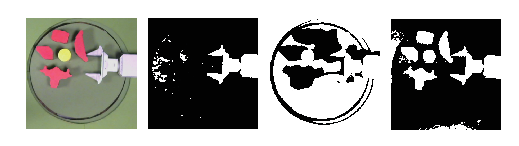
\includegraphics{f_figs/binary_segment.eps}

\caption{\footnotesize Example of how the binary mask applied to each RGB channel affects the input data. As can be seen
it reduces the range of each channel's pixel value from the range of [0,255] to [0,1], increasing robustness to small
lighting condition changes.  }

\label{fig:b_seg}
\end{figure}



\begin{figure}[t]
\centering

\includegraphics{f_figs/robot.eps}

\caption{\footnotesize  Shown above is a Zymark robot. The robot consists of an 3DOF arm in a planar workspace. It is able to extend its arm and rotate about a fixed base. The robot can also open and close its gripper.}

\label{fig:robot}
\end{figure}

\begin{figure}[t]
\centering
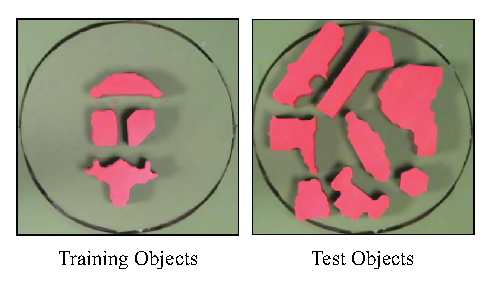
\includegraphics{f_figs/shapes_set.eps}

\caption{\footnotesize  The Training objects on the right are the four objects used in training. The test objects on the
left represent represent objects that were added in our test configurations. Every test configuration contained at least
one of the objects on the right.}

\label{fig:shape_set}
\end{figure}


\begin{figure}[t]
\centering
\includegraphics{f_figs/succes_measure.eps}

\caption{\footnotesize  Right: examples of training configurations we presented to the robot. The shapes were arranged
around the goal object in different poses and in different parts of the workspace. At test time, we considered similar configurations but 
added some unknown objects not present in the test set. }
\vspace*{-20pt}
\label{fig:suc_meas}
\end{figure}

We discuss our experimental setup and test the performance of using a supervisor hierarchy versus a baseline approach
with one supervisor. We then evaluate the quality the Crowd-Source supervisors. 

\subsection{Experimental Setup}
We work with a Zymark robot to perform a grasping in clutter task. The robot, shown in Fig. \ref{fig:robot}, has a 3
dimensional internal state of base rotation, arm extension and gripper opening width. The robot is commanded via position 
control with a tuned PID controller. We used
relative state control because this enabled us to easily enforce stay out zones for safety
and to register control signals to the labeling interface in Fig. \ref{fig:overlays}. We utilize the two main rotational joints of the
robot as degrees of freedom which are controled by a neural network policy $\pi_{\theta}$ trained on image data taken by
an overhead Logitech C270 camera. Examples of images from the camera can be seen in Fig. \ref{fig:teaser}.

We consider objects made of Medium Density Fiberboard with an average 4" diameter. The objects used to form clutter are
painted red while the goal object is a yellow cylinder. The robot workspace consists of a disk region which is
surrounded by an elevated plate constraining the objects to the workspace and prohibiting them from being sweeped off
the workspace, thus adding to the difficulty of the task.

Our policy $\pi_{\theta}$ is represented as a deep neural network, which was trained using
TensorFlow~\cite{tensorflow2015-whitepaper}. Our network architecture consists of 1 convolutional layer with 5 channels
and filters with size 11x11, a fully connected layer with an output of 128 dimensions and a final layer that maps to a
four dimensional control signal. We used ReLus to separate the different layers and a final tanh on the output to scale
the output between -1 and 1. Each policy runs for a total of $T=100$ timesteps.

The control examples were scaled between 1 and -1 for each dimension independently. To be robust to lighting and reduce
the dimensionality of the problem, we applied a binary mask to each channel of the 250x250 RGB video frames setting
values above 125 to one and 0 otherwise. Each channel is shown in Fig. \ref{fig:b_seg}.
The policy $\pi_\theta$ outputs delta position control signals for a given input video frame.
Originally we considered also controlling two additional degrees of freedom of the arm: a turn-table motor controlling
the rotation of the disc workspace and the single degree of freedom of the robot gripper. However, in initial
experiments controlling the turn table proved unintuitive and was rarely used by human supervisors and the gripper degree of freedom was only used at the end of a policy. As a result, we labeled these output degrees of freedom with zero and instead automatically closed the gripper
at the final T=100 timestep. The joint controls were limited to $\pm 15$ degrees for rotation and $1$ cm for the
extension degree of freedom.

To determine our network architecture we preformed a search over 40 different architectures trained after 400 iterations
with a batch size of 200. The set of architectures consisted of different network architectures in terms of
convolutional layers, fully connected layers and size of each one as well as different gradient descent momentum
terms used in learning, and weight initialization schemes. In finding an architecture, we trained all networks on a dataset of 6K images labeled with the Algorithmic Supervisor on a Nvidia Tesla K40 GPU, which is able to train each network in an average of 10 minutes.  

To test the performance of a policy, we created a test set composed of 20 different configurations each containing
objects that were not in the training set.  The training objects and test
objects introduced during testing are shown in Fig. \ref{fig:shape_set}. The test set configurations varied by placing
unknown objects from Fig. \ref{fig:shape_set} in addition to the objects we trained on. Examples of training and test configurations are shown in Fig. \ref{fig:suc_meas}.  We measure success by whether the object was in the gripper at the final timestep. 
Per iteration of DAgger, we roll out 20 trajectories which corresponds to 2000 video frame images. Thus 100 robotic trials correspond to 5 iterations of DAgger.

\subsection{Hierarchical Supervisors}

\begin{figure*}[t]
\centering
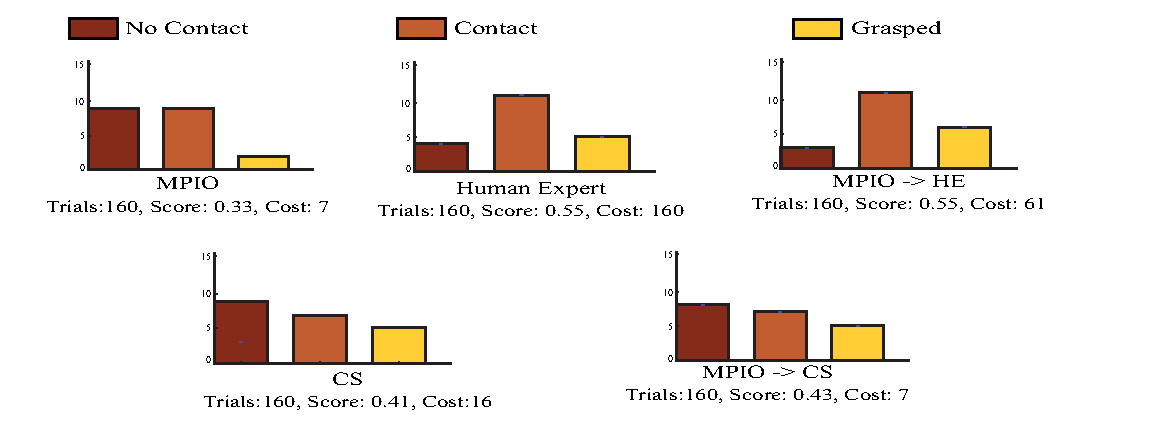
\includegraphics{f_figs/results.eps}

\caption{ \footnotesize The \% of Grasp Success Score and cost of each policy trained with a supervisor is reported. The bar graphs
show how many successful and failed grasps in clutter occurred. The top row 
reports results for the Algorithmic and human expert supervisor in isolation and a hierarchical experiment
utilizing only the algorithmic and human expert supervisor.
The bottom row corresponds to experiments testing a crowdsourced supervisor: Left: Crowdsourced supervisor training in
isolation, Right: A hierarchy of Algorithmic and Crowdsourced supervisor.}

\label{fig:perf_results}
\end{figure*}

We first test that using a hierarchy of supervisors can reduce total cost needed to train a policy, but still maintain
similar performance . We compare having only a Algorithmic Supervisor for a fixed amount of data to having only an Human Expert,
and to having the hierarchy of both. The non-hierarchical policies trained with the human expert supervisor only for
160 demonstrations or only the AS supervisor for 160 demonstrations.  The policy trained with a hierarchical supervisor
first receives  100 demonstrations from the AS supervisor and  60 demonstrations from the expert supervisor. 

Our results, shown in Fig. \ref{fig:perf_results}, show that the policy trained with just the Algorithmic Supervisor
achieves a score of $30\%$, the policy trained with just the Human Expert Supervisor achieves $55\%$ and the policy
trained with a hierarchy of supervisor achieves $60\%$.  Thus, the hierarchical supervisor and expert supervisor achieve
approximately the same performance. However, training with a two step hierarchy of both yields a $40\%$ reduction in
cost incurred compared to the policy trained with only an expert supervisor. Thus indicating that by using a hierarchy of supervisors, we can reduce the cost of training a policy and achieve similar performance to the Human Expert Supervisor.

\subsection{Quality of Crowdsourced Supervisor}
We next evaluate the potential of a  crowdsourced supervisor for a being part of the hierarchy. Thus, we perform an
experiment using the Amazon Mechanical Turk (AMT) platform described in Sec. \ref{sec:hier}. We  first test how well a crowdosurce supervisor
performs as part of a hierarchy of supervisors. We trained a policy with 100  demonstrations provided by the algorithmic
supervisor, then had 60 demonstrations provided by AMT workers. We also compare how well the crowdsource supervisors
performs in isolation, by having them provide all 160 demonstrations.

Our results, shown in Fig. \ref{fig:perf_results}, indicate that the policy trained with just the crowdsourced supervisor achieves
a score of $35\%$. The policy trained with the hierarchical crowdsourced and algorithmic supervisor obtained a score of
$45\%$ on our test set compared to $60\%$ with the motion planning and expert supervisors hierarchy. The total cost of
using only crowdsource supervisor was 15, while the hierarchical supervisor was 7. 

In total, we utilized 44 AMT workers and asked them to provide examples for a single rollout and then if they passed
quality check asked them if they wanted to exit or continue for an additional \$$0.12$ per demonstration. We found only
21 AMT workers were able to pass the quality check and continue providing demonstrations. On average a worker would
provide 4 demonstrations before exiting the AMT HIT. {\color{blue} [WHAT IS HIT?]}

\subsection{Advancing in the Hierarchy}
We further test how to advance between supervisors in the hierarchy. We examine three different strategies for dataset
management when changing supervisors 1) aggregating the dataset of the data collected with both supervisors 2)
transferring only the weights of the nerural network policy or $\theta$ vector between the supervisors and removing the
previous supervisors' demonstration dataset completely 3) transferring only the weights of the neural network policy but
adding the values output by $\pi_\theta(\bx)$  instead of $\tilde{\pi}_m(\bx)$ at parts of the states visited that the
current supervisor is in close agreement with as measured by the following $||\tilde{\pi}_m(\bx) - \pi_\theta(\bx)||^2_2
< 0.01$. Thus, acting as a regularization on the optimization since stochastic gradient on a section of the mini-batch update would be zero for examples where the next supervisor agrees with the previous. 

We compare each strategy on a hierarchy of an algorithmic supervisor trained with 100 iterations and then advancing to a human expert supervisor trained with 60 iterations.  Our results reported in Fig.\ref{fig:cost_result}, show that aggregation strategy achieves $15\%$, the weight transfer strategy achieves $55\%$ and the regularized stochastic gradient update strategy achieves $65\%$. Thus, suggesting that techniques to help the policy remain close to the previously trained supervisor are useful for effectively switching between supervisors.   
An issue arises though when performing these iterations because now the current dataset $\mathcal{D}_{K_m}$ has examples from a different supervisor that receives a smaller expected cumulative reward. 

%This could cause a learning algorithm to try and fit to contradictory examples  and be worse than either supervisor trained with \cite{scholkopf2002learning}.
%We are thus interested in only remembering the current $\theta_{m,K}$ weight parameters as we transition between
%different supervisors. Thus, we propose only performing DAgger for each individual supervisor in the
%hierarchy and use the resulting weight vector to bootstrap the learning of the next supervisor. We found empirically
%in Sec. \ref{sec:Exp} that it is also beneficial to add the new dataset the states and controls applied by the current
%policy $\pi_{\theta_{m,k}}$ that the current supervisor agreed with by some euclidean distance
%$\tilde{\epsilon} = 0.01$. Thus, acting as a regularization on the optimization since stochastic gradient on a section of the min-batch update would be zero for examples where the next supervisor agrees with the previous. 


\begin{figure}[t]
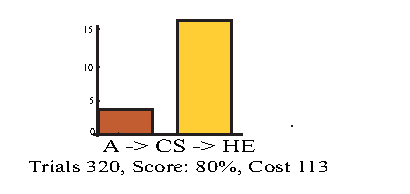
\includegraphics{f_figs/big_data.eps}
\centering 
\caption{ \footnotesize  The performance and cost of the policy trained on the full hierarchy with of Algorithmic, Crowdsourced and Human Expert. The policy achieves a success rate or score of $80\%$ success. The total cost though after 320 trials is only 113.  }
\vspace*{-20pt}
\label{fig:big_data}
\end{figure}

\subsection{Scaling the Hierarchy}
Here, we ran our algorithm on a hierarchy with 3 supervisors: Algorithmic supervisor, crowdsourced and human
expert. We ran each policy until we observed the pay out in terms of reward achieved was not increasing. This results in
AS for 100 demonstrations, crowdsourced for 120 demonstrations and human expert for 100 demonstrations. Thus resulting
in 320 trials on the robot and approximately 22,000 images annotated by control supervision labels. Note however that
fewer images had non-zero delta-control labels because the human supervisors only labeled when confident in their
decisions. {\color{blue} [HOW MANY?]}

The results of our trained policy, as shown in Fig. \ref{fig:big_data}, demonstrate that by leveraging a hierarchy we are able to achieve a score of $80\%$ with a cost of only 113. We note that policy trained with the human expert supervisor, which incurred a cost of $160$, was only able to achieve a score of $55\%$. 

Investigating the learned policy, we observed that it appears to find gaps in between the clutter objects and sweeps
left to right,  until the objects are pushed apart and then moves towards the goal object, as illustrated in Fig.
\ref{fig:teaser}. We noticed that the magnitude of the sweeping motion appeared anti-proportional to the size of the gap in
the between the cluttered objects. Small gaps tended to cause a high frequency of sweeping while for large gaps the
robot appeared to sweep away objects in a single motion.

While our policy showed improved performance when trained using a hierarchy, failure modes persisted in our test
configurations are shown in Fig. \ref{fig:failure_modes}. The cause of the failure modes are either that the robot
sweeps too far and jams the objects against the inscribed circle around the workspace or an obstacle object was caught
in the gripper while being pushed. At present, it is unclear how well these results will generalize to very different configurations 
of objects.

\begin{figure}[t]
\centering 
\includegraphics{f_figs/failure_modes.eps}

\caption{\footnotesize The four failure modes in our test set on the fully trained policy. On the left the robot sweeps
to far and the collision objects jam up against the edge of the work space. On the right, both the banana-shaped object
and the boot-shaped object are prone to get entrapped in the gripper during pushing and prevent the gripper from reaching the circle.  }
\label{fig:failure_modes}
\end{figure}


\begin{figure}[t]
\centering 
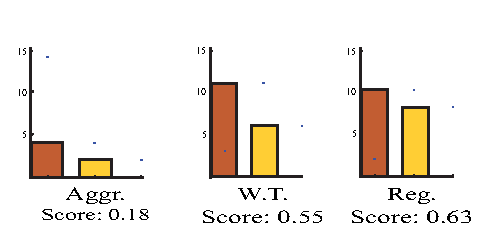
\includegraphics{f_figs/cost_result.eps}

\caption{\footnotesize The performance of each policy trained with a different data management strategy is reported. The
bar graphs shows the breakdown in terms of situations the policy encountered on the test set. Each policy was trained
with the AS to Human Expert hierarchical supervisor. From left to right is the following data management strategies: Dataset Aggregation, Weight Transfer and Regularization. Regularization achieves the highest performing score of (0.65) }
\label{fig:cost_result}
\end{figure}

\section{Discussions and Future Work}
Our results suggest that learning to grasp in clutter can be more cost-efficiently learned by employing a hierarchy of
supervisors. In future work, we intend to investigate algorithmic approaches to determining how to appropriately select
the next supervisor in a hierarchy automatically, which we believe will require a significant scaling of the number of
training iterations due to the sparsity of the current data set. While our current strategy worked well empirically, it remains to be 
investigated how this approach can be utilized in different application domains and higher degree of freedom robots.
A current challenge of our setup appears to be related to a lack of fine motor precision. 
Our current supervisors do not have the ability to give fine motor control corrections. Furthermore, the use of more
sophisticated analytical methods as supervisors might enable better performance. 
Further information, video and code can be found at the following \url{http://berkeleyautomation.github.io/HierSupCASE/}. 




 \section{Acknowledgments} 
This research was performed in UC Berkeley's Automation Sciences Lab under the UC Berkeley Center for Information Technology in the Interest of Society (CITRIS) "People and Robots" Initiative. This work is supported in part by the U.S. National Science Foundation under Award IIS-1227536, NSF-Graduate Research Fellowship, by the Knut and Alice Wallenberg Foundation and the National Defense Science and Engineering Graduate Fellowship Program. We thank Steve McKinely and Meng Guo for help in building the hardware setup.  

  
\bibliographystyle{IEEEtranS}
\bibliography{references}



\end{document}
%\subsection{Hierarchies} If the robot could learn the policy  perfectly, this state density would match the one encountered in user examples. But if the robot makes an error, that error changes the distribution of states that the robot will visit, which can lead to states that are far away from any examples and difficult to generalize to~\cite{pomerleau1989alvinn}. This motivates iterative algorithms like DAgger, which iterate between learning a policy and the supervisor providing examples. We  introduce the concept of their being a set of supervisors each with an associated cost and skill level. Denote $\tilde{\pi}_M$ the most skilled and costly supervisor in this set. This supervisor could for example be a person with a Phd in machine learning and robotics. We formally define how each supervisor in the set is related to each other in Sec. \ref{sec:hS}.  Every time a supervisor is queried a cost, $C_m$, is incurred this could be an hourly pay rate or computational time. While Eq. \ref{eq:LFD_obj} is the primary objective of our algorithm a secondary objective is to reduce the cumulative cost associated with training the robot. Thus, we are interested in solving the following objective

%where $J$ is the number of queries need to satisfy the constraint on expected surrogate loss, $C_{m,j}$ denotes the cost incurred by querying the supervisor at that iteration and $\epsilon$ is a user-defined threshold on how close robot policy is to match the highest quality supervisor. We present our algorithm, LEATHERMAN, which aims to solve Eq. \ref{eq:bugjet_LFD_obj}.
 

%\subsection{Hierarchy of Supervisors}\label{sec:hS} Instead of one  supervisor,we propose a hierarchy  of $M$ supervisors where for each supervisor $\tilde{\pi}_m$, there is an associated expected cumulative reward $R_m = \int \sum^T_{t=1} r(\mathbf{x}_t, \tilde{\pi}_m(x)) p(\tau |\tilde{\pi}_m)d\tau$, where $p(\tau |\tilde{\pi}_m)$ denotes the average distribution of states the supervisor encounters. We also denote some measure of cost $C_m$ that is ascribed to the supervisor, such as computational time or monetary expense. Generally the rank of supervisors in terms of cost is equivalent to the rank of supervisor in the terms of expected cumulative reward. Thus, the least costly supervisor will receive the lowest expected cumulative reward. 

%Additionally for two supervisors $\tilde{\pi}_m$ and $\tilde{\pi}_{m+1}$ to be in the hierarchy, they must only disagree in expectation on a subset of the work space to some precision $\tilde{\epsilon}$. Denote the set of states two supervisors disagree as $\mathcal{X}_{m,m+1} = \lbrace \mathbf{x} | ||\tilde{\pi}_m(\mathbf{x}) - \tilde{\pi}_{m+1}(\mathbf{x}) ||^2_2 > \tilde{\epsilon} \rbrace$ .We enforce the condition $\mathcal{X}_{m,m+1} \subset \mathcal{X}$ because if two supervisors never provided the same examples then all states would have to be relabeled by the next supervisor in the hierarchy. 

%We formally define an ordering on supervisors:

%\begin{definition} Two supervisors $\tilde{\pi}_m$ and $\tilde{\pi}_{m+1}$ are in a hierarchy if  $C_m < C_{m+1}$  and  $\mathcal{X}_{m,m+1} \subset \mathcal{X}$ \end{definition}

%Violation of this definition could result in no additional benefit from the LEATHERMAN algorithm or potentially worst a higher budget incurred than without using a hierarchy of supervisors.
